\documentclass[twocolumn,twoside,showpacs,preprintnumbers,superscriptaddress,amsmath,amssymb,prc,nofootinbib]{revtex4}


% \documentclass[preprint,preprintnumbers,superscriptaddress,amsmath,amssymb]{revtex4}
 %\documentclass[preprint,preprintnumbers,amsmath,amssymb]{revtex4}


\usepackage{cases}
\usepackage[normalem]{ulem}
\usepackage{amsmath}
\usepackage{subcaption}
% \usepackage{subfig}
 \usepackage{CJK}
 %\usepackage{ccmap}
 \usepackage{txfonts}
 \usepackage{mathrsfs}
 \usepackage{amssymb}
 \usepackage{graphicx}% Include figure files
 \usepackage{dcolumn}% Align table columns on decimal point
 \usepackage{bm}% bold math

 \usepackage{floatflt}
 \usepackage{float}
 \usepackage{siunitx}
 \usepackage{rotating}
 \usepackage{tikz}
\usepackage{physics}
 \usepackage{multirow}
 \usepackage[bookmarksnumbered,bookmarksopen,colorlinks,citecolor=blue,linkcolor=blue]{hyperref} %
 %\usepackage{booktabs}
 \usepackage{epsfig,graphics,psfrag}
%  \usepackage{sidecap}

 %\bibliographystyle{apssamp}
 \bibliographystyle{apsrev}

\def\esym{$E_{\rm sym}(\rho)$}
\def\thu{Department of Physics, Tsinghua University, Beijing 100084, China}
\def\riken{RIKEN Nishina Center, Hirosawa 2-1, Wako, Saitama 351-0198, Japan}
\def\gxnu{College of Physics and Technology, Guangxi Normal University, Guilin 541004, China}
\def\gxkl{Guangxi Key Laboratory of Nuclear Physics and Technology, Guangxi Normal University, Guilin 541004, China}

\begin{document}
      
 \title{Simulation studies of the isovector reorientation effect of deuteron scattering on heavy target}

 \author{Baiting Tian}
 \email[Corresponding author: ]{tbt23@mails.tsinghua.edu.cn}
 \affiliation{\thu}
 
 
 \author{Boyuan Zhang}
 \affiliation{\thu}

\author{Dawei Si}
\affiliation{\thu} 

\author{Sheng Xiao}
\affiliation{\thu} 

\author{Yijie Wang}
\email[Yijie Wang:]{yj-wang15@tsinghua.org.cn}
\affiliation{\thu}

\author{Tadaaki Isobe}
\email[Tadaaki Isobe:]{isobe@riken.jp}
\affiliation{\riken}


\author{Hideaki Otsu}
\email[Hideaki Otsu:]{otsu@ribf.riken.jp}
\affiliation{\riken}

\author{Li Ou}
\email[Li Ou:]{liou@gxnu.edu.cn}
 \affiliation{\gxnu}
 \affiliation{\gxkl}

\author{Zhigang Xiao}
\email[Zhigang Xiao:]{xiaozg@tsinghua.edu.cn}
\affiliation{\thu}

\date{\today}

% \footnotetext[*]{Zhigang Xiao. E-mail: xiaozg@tsinghua.org.cn} 
% \footnotetext[\dagger]{Tadaaki Isobe. E-mail: isobe@riken.jp
% } 


\begin{abstract}

The isovector reorientation (IVR) effect of deuteron scattering on heavy target provides a novel means to probe the nuclear isovector potential, which gives rise to the nuclear symmetry energy.  The simulation studies on the experimental measurement of IVR  effect using the SAMURAI terminal at RIKEN Nishina center have been performed to demonstrate the feasibility of the experiment. By introducing a well-designed polarimeter to detect the $\mathrm{p}(\vec{\mathrm{d}}, \mathrm{d})\mathrm{p}$ elastic scattering,  monitoring of the tensor polarization of the deuteron beam can be implemented. The protons and neutrons produced by the breakup of polarized deuterons scattering off heavy targets are designed to be measured by proton drift chamber (PDC) combined with the SAMURAI magnet and NEBULA detector, respectively. The detector responses are simulated using Geant4 framework, where the events of the deuteron elastic breakup are generated by an Improved Quantum Molecular Dynamics model. The results of reconstructing the deuteron breakup events demonstrate the feasibility of detecting the IVR effect at SAMURAI with both longitudinal and transverse tensor polarized deuteron beams with a polarization degree of approximately 80\%.
%at approximate 80\% polarization. 

\end{abstract}


\keywords{Analysing Power; Isovector Reorientation Effect;  Tensor polarization; ImQMD; Deuteron-induced Reaction}

 \maketitle
 
\section{Introduction} 




The symmetry energy characterizes the isospin-dependent part of the nuclear equation of state, quantifying the energy cost associated with neutron-proton asymmetry \cite{li2008recent,danielewicz2002determination,Li2021}. The density dependence of the symmetry energy, \esym, has drawn increasing attention from both nuclear physics and astrophysics communities. However, the stiffness of \esym~ still suffers from significant uncertainty, particularly at supra-saturation densities \cite{Li:2019xxz}. Recently, enormous progress has been made from heavy ion experiments \cite{Tsang:2004zz,SpiRIT:2021gtq,Xiao:2008vm,Zhang:2017xtk} and observations of gravitational waves generated by neutron star merger \cite{LIGOScientific:2017vwq,LIGOScientific:2018cki}, as well as the combination of the two \cite{Tsang:2023vhh,Huth:2021bsp}. Further elaborations are still ongoing in searching new probes of \esym \cite{Wang:2021mrv,Wang:2022ysq,Wang:2023kyp}.

Using Hugenholtz–Van Hove theorem \cite{Hugenholtz:1958zz}, the relationship between symmetry energy and single particle potential ($U_{\mathrm{n/p}} = U_0 \pm U_{\mathrm{sym}}(\rho, k_{\mathrm{F}})$) can be easily derived. We can decouple the symmetry energy into several parts related to the single-particle potential and Fermi kinetic energy \cite{PhysRevC.82.054607} 
\begin{align}\label{Esym2}
E_{\rm sym}(\rho) &= \frac{1}{6} \frac{\partial
[t(k)+U_0(\rho,k)]}{\partial k}\Big|_{k_{\rm F}} \cdot k_{\rm F} + \frac{1}{2}
U_{\rm sym}(\rho,k_{\rm F})\nonumber \\ 
&=\frac{1}{3} t(k_{\rm F}) + \frac{1}{6}
\frac{\partial U_0}{\partial k}\Big|_{k_{\rm F}}\cdot k_{\rm F} +
\frac{1}{2}U_{\rm sym}(\rho,k_{\rm F})  \\
&= \frac{k_{\rm F}^2}{6m^*_0 (\rho,k_{\rm F})} + \frac{1}{2} U_{\rm sym}(\rho,k_{\rm F}), \nonumber
\end{align}
where $t(k_{\mathrm{F}})$ is the nucleon kinetic energy at the Fermi momentum $k_{\mathrm{F}} = \left( \frac{3\pi^2\rho}{2} \right)^{1/3}$ at the symmetric nuclear matter density $\rho$. Equation \ref{Esym2} shows that the microscopic origin of the symmetry energy is the difference between the neutron and proton Fermi surfaces. For the isoscalar potential $U_0(\rho, k)$, information on its density and momentum dependence has been obtained from high-energy heavy-ion collisions (e.g., see Ref. \cite{danielewicz2002determination}). While existing data constrain its behavior to some extent, significant uncertainties persist in high-momentum and high-density regimes. In contrast, the isovector potential $U_{\mathrm{sym}}(\rho, k)$, particularly at extreme densities and momenta, remains poorly constrained. This potential has been identified as a critical parameter for resolving ambiguities in the high-density behavior of the symmetry energy \cite{xu2011analytical,chen2012single,li2008recent}. At saturation density, the isoscalar effective mass $\frac{m_0^*}{m} = 0.70\pm0.05$, and the isovector potential $U_{\rm sym}(\rho_0,k_{\rm F})=28.7 \pm 7.8~\mathrm{MeV}$ \cite{li2013constraining,li2015neutron}. Therefore, the challenge of excluding the interference of isoscalar forces in heavy-ion experiments while extracting the characteristics of isovector forces has become critical.
  
The isovector reorientation (IVR) effect effectively mitigates the influence of the isoscalar potential, enabling the extraction of isovector information with high sensitivity \cite{PhysRevLett.115.212501,PhysRevC.101.024603}. As shown in Fig. \ref{fig:ivr-view}, in the peripheral scattering of a polarized deuteron beam on a heavy target, the isovector force, which is attractive to protons and repulsive to neutrons, acts like a torque on the deuteron, inducing an additional rotation of the latter. Consequently, the subsequent breakup incorporates the rotational effect, which exhibits high sensitivity to the isovector force. Detailed simulations demonstrate that the angular
distribution of the correlated neutron and proton from the deuteron breakup is highly sensitive to the isovector potential, yet insensitive to the isoscalar nuclear potential. The experimental observable is straightforward to implement: measuring the angular distribution of the relative momentum vector between neutrons and protons arising from the breakup of a polarized deuteron. This observable acts as a probe with exceptional sensitivity to the symmetry energy in regions of low nuclear density. By employing this probe, the uncertainties in the density dependence of the symmetry energy can be effectively constrained.
  
  
   \begin{figure}
    \centering
    \includegraphics[width=0.45\textwidth]{./isovector_reorientaton.png}
    \caption{The schematic view of the isovector reorientation effect of a polarized deuteron scattering on a $^{124}$Sn target, followed by the elastic breakup. The inset presents the momentum vectors to be used in the following analysis.}
    \label{fig:ivr-view}
\end{figure}
  
Among various research and development (R\&D) works, two key issues have to be addressed before conducting the experiment at SAMURAI, RIKEN Nishina center.  One is the monitoring of the polarized deuteron beam, the other is the design (and optimization) of the detector setup to measure the breakup of the polarized deuteron scattering on heavy target, which carries the IVR effect. These two issues can be elucidated by simulation studies, which make the current paper. The remainder of this paper is organized as following. In Section \ref{sec:exp_plan}, we outline the experimental plan and describe the simulation methods employed in this study. Section \ref{sec:MonitorPol} focuses on the monitoring of the polarized beam, where we define tensor polarization and introduce two monitoring options. Moreover,   the design of the polarimeter and  the simulation results for beam monitoring are presented. Section \ref{model_desc} describes the ImQMD transport model as the event generator in our simulations. Section \ref{sec:AngDistribution} present the simulation of the detector response at SAMURAI and the event reconstruction. We detail the detector setup, target position optimization, and the responses of both neutrons and protons, along with the background simulation and the beam dumper. Additionally, we observe the IVR effect within the current experimental design. Finally, Section \ref{sec:Conclusion} provides the conclusion and outlooks of the study.
  


\section{A brief introduction to the beam experiment}
\label{sec:exp_plan}

The experimental setup is specifically optimized to measure the isovector reorientation effect in deuteron scattering on heavy targets. Figure \ref{fig:exp_plan} presents the overview of the beam line and detector arrangement, highlighting the strategic placement of key components to maximize detection efficiency and minimize background. The deuteron beam is polarized and accelerated to 190 MeV/u. The tensor polarized beam is provided by the polarized ion source and accelerated by the AVF and RRC successively, and then by SRC through the IRC bypass transport beam line. The spin symmetry axis of the deuteron beams is controlled by the Wien Filter prior to acceleration. Single-turn extractions are required for the three cyclotrons to maintain polarization amplitudes during acceleration. The polarization of the deuteron beam
is typically 80\% of the theoretical value\cite{sakamoto2016acceleration}.

\begin{figure*}
    \centering
    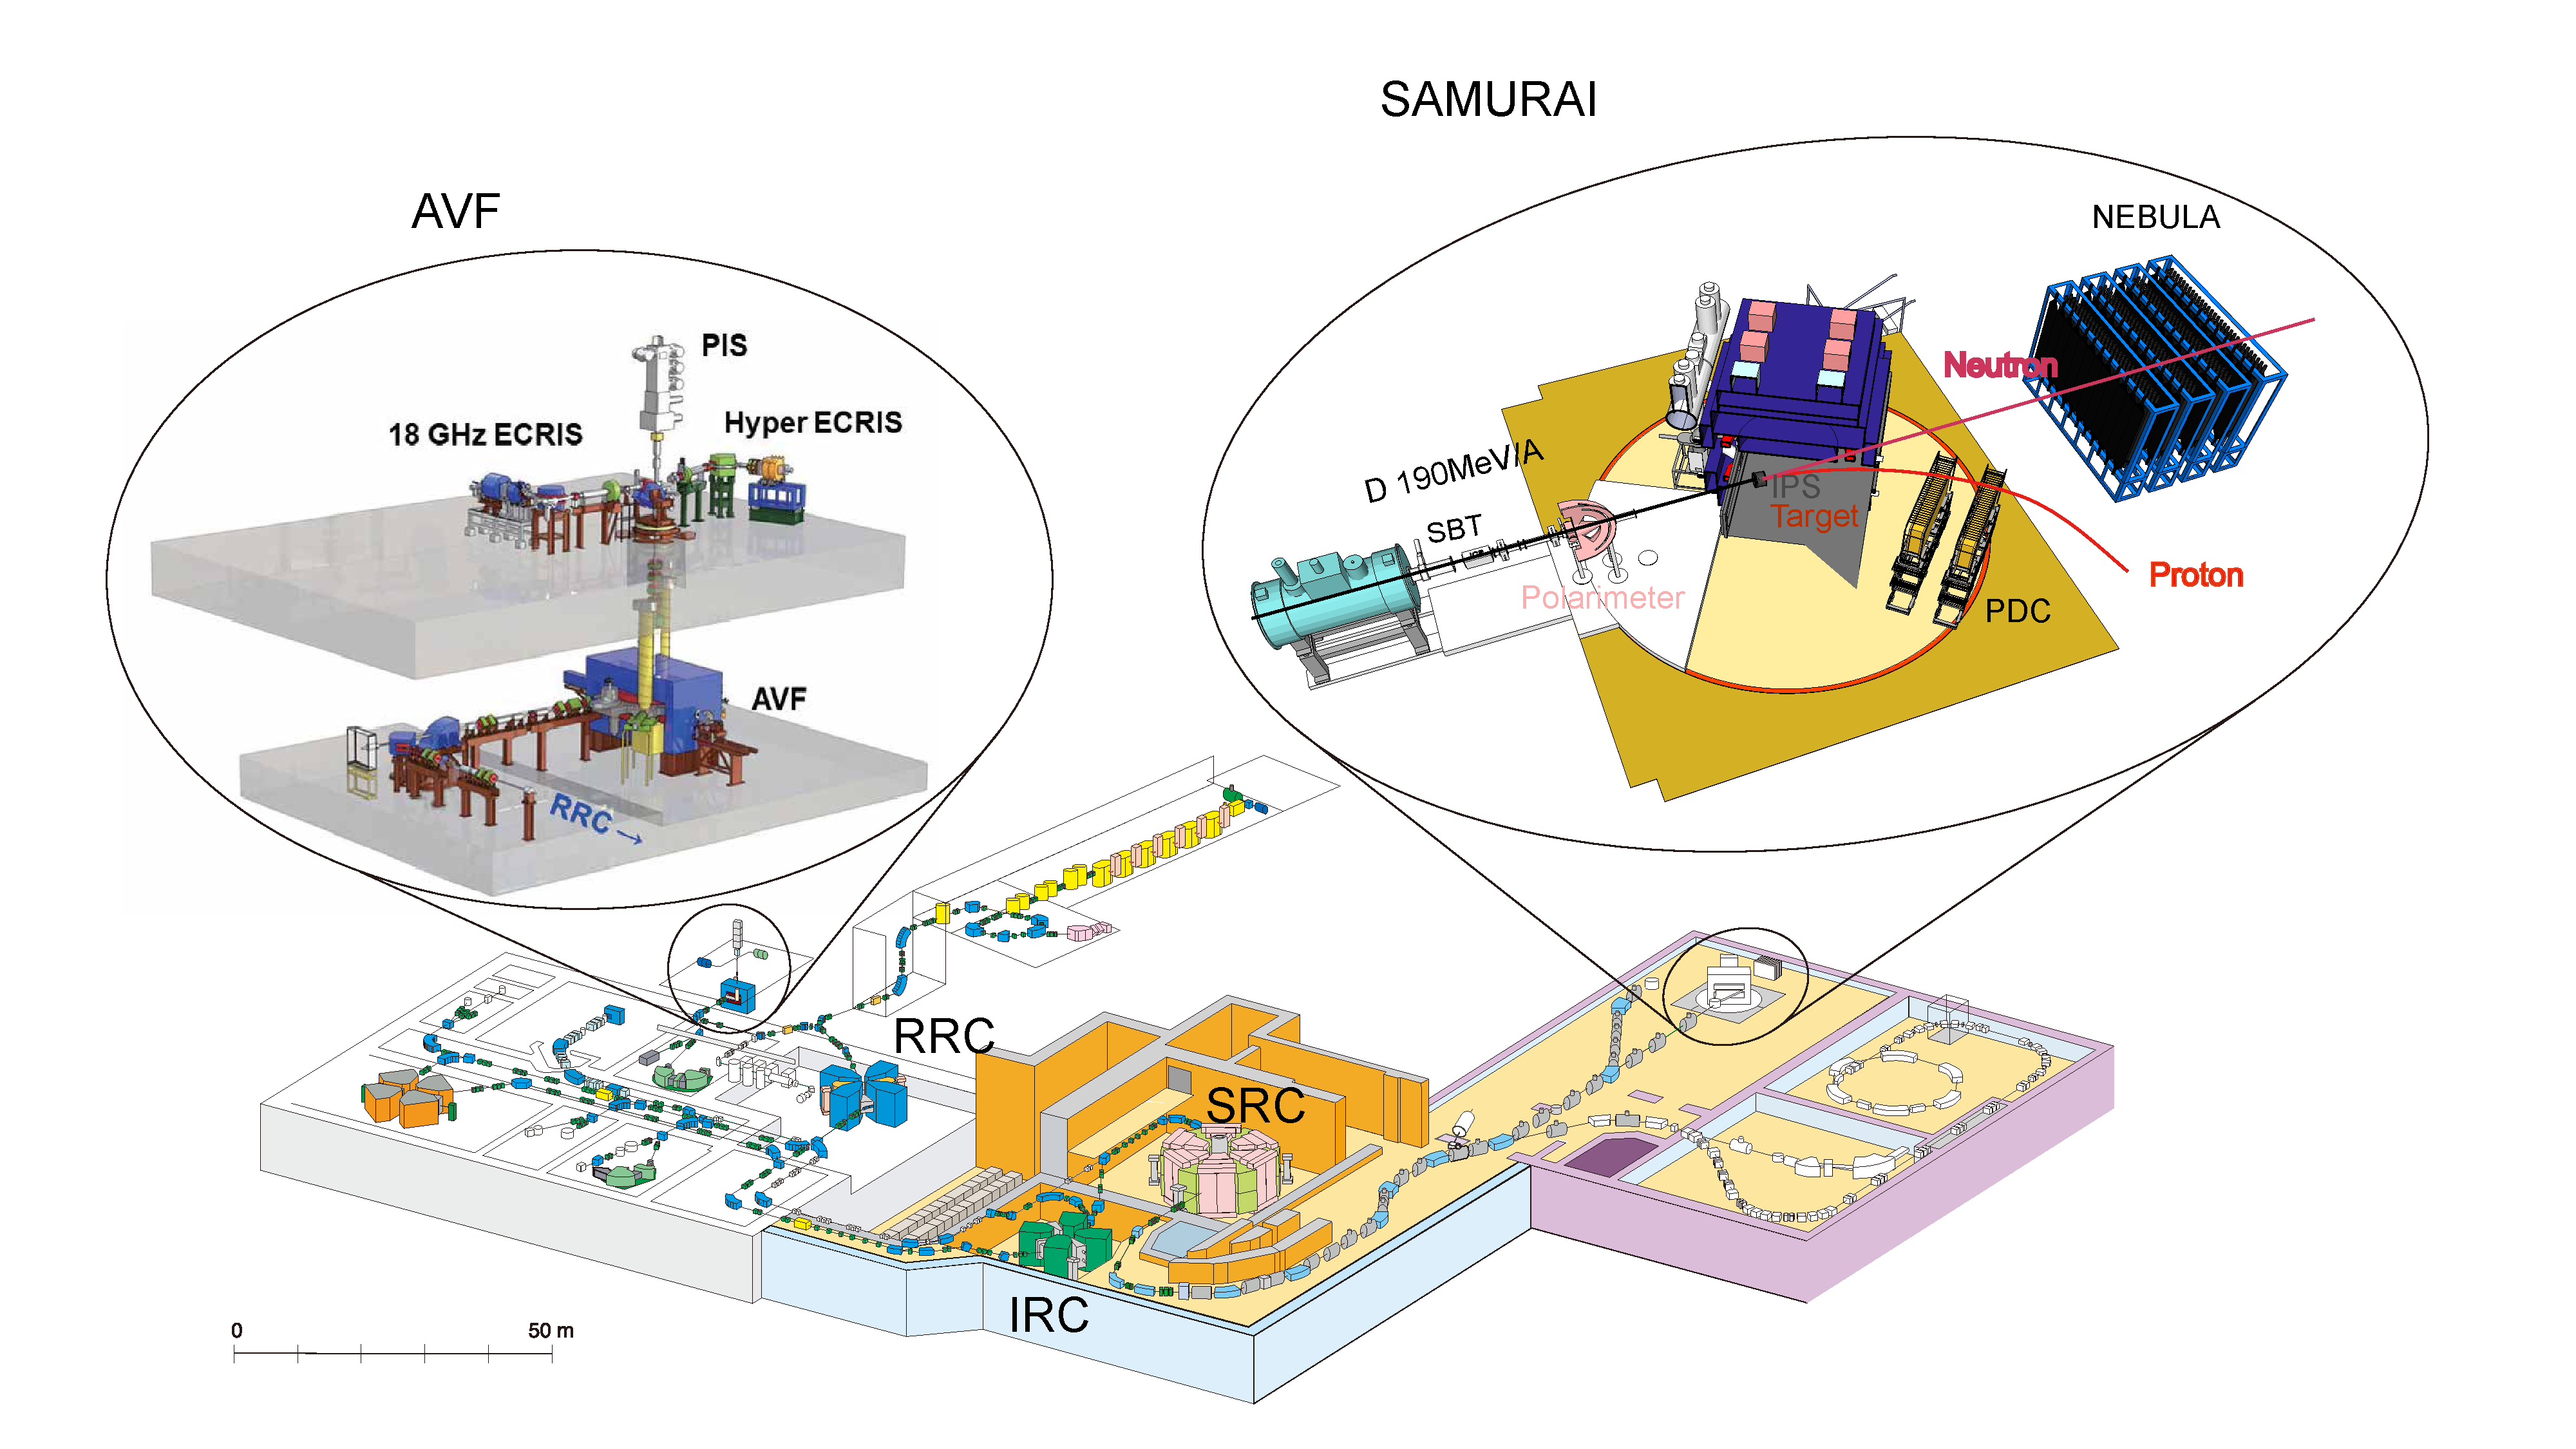
\includegraphics[width=\textwidth]{./schematic_of_beamline.pdf}
    \caption{The bird's-eye view of the experiment.}
    \label{fig:exp_plan}
\end{figure*}



The experimental IVR effect is detectable  in longitudinal ({$p_{zz}$}) and vertical ({$p_{yy}$}) polarization conditions. The deuteron-induced scattering involves both nuclear and Coulomb interactions. To differentiate nuclear and Coulomb effects, it is planned to use three different targets, $^{112}\rm{Sn}$, $^{124}\rm{Sn}$, and $^{208}\rm{Pb}$. The  $^{124}\rm{Sn}$ and the $^{208}\rm{Pb}$ have the same neutron abundance ( $N/A$ = 0.60 and 0.61, respectively) but different atomic charge,
therefore the isospin effect is alike and the difference is expected due to the Coulomb force.

We intend to optimize the reaction vertex in the SAMURAI dipole to
make the best use of the coverage of the detectors. According to the Improved Quantum Molecular Dynamics (ImQMD) model
calculations, for the scattering events with $b=7\sim9\,\mathrm{fm}$
which is the range showing the most sensitivity of IVR effect on the $\gamma$ parameter, which is introduced to mimic different density dependence of $E_{\rm sym}(\rho)$, the most probable direction of the breakup neutrons is not very close to $\theta=0{^\circ}$.
Considering that NEBULA is difficult to move, in order to measure
the neutrons in the most favorable range of $\theta_{\mathrm{n}}$,
it is suggested to place the target upstream of the magnet, at a distance of 3 meters from the center of the magnet, which ensures that the range of $-10{^\circ}\le\theta_{\mathrm{n}}\le10{^\circ}$ is covered for the most probable neutron emissions.

As for the SAMURAI magnet, we  choose $B=1.2\,\mathrm{T}$ and
the $30{^\circ}$ configuration, which fits mostly our experimental
purpose. In addition, we do not require the magnet chamber to be in
vacuum, since the beam trajectory is influenced little by the air
at the current beam energy. By removing the downstream exit window of the SAMURAI chamber, we
have a wider range of exit angle for both neutrons and protons. 
According
to the simulation results, the reorientation effect can be observed
for both $z$-polarization ($p_{zz}$) and $y$-polarization ($p_{yy}$). Therefore,
we prefer to use either the $z$-polarization or $y$-polarization in our
experiment, depending on the machine condition. The unreacted deuteron beam will be collected
by the beam dumper, which is surrounded by a water tank to shield the neutron background radiation.

To achieve the experimental goal, the detector system is arranged with a polarimeter and a veto detector upstream of the target to monitor deuteron polarization and suppress inelastic background, respectively. Downstream of the target, protons from deuteron breakup are detected by the proton drift chamber (PDC) backed by a time-of-flight (TOF) array of plastic scintillators, while neutrons are detected by the NEBULA array. The PDC is positioned 3 meters from the target, and NEBULA is placed 7.3 meters from the target, ensuring optimal detection efficiency for both protons and neutrons.





 
\section{Monitor the tensor polarization }
\label{sec:MonitorPol}

For this experiment, a polarized deuteron beam is essential. 
Because of the unpolarized deuteron beam, the random orientation will average out the differences in the proton-neutron angular distribution.

To ensure accurate measurements, we monitor the deuteron beam's polarization using a method based on d-p elastic scattering. This involves measuring the cross-sections at different angles to confirm the polarization state. While the theoretical framework for polarized nuclear reactions is well established and experimental techniques for monitoring $p_{y'y'}$ are available, the direct measurement of $p_{z'z'}$ remains unexplored. This work addresses this gap by developing a robust monitoring mechanism for $p_{z'z'}$. To avoid misunderstandings caused by different notational conventions, we start from the most fundamental principles and derive our polarization monitoring mechanism in detail.


\subsection{Definition of  the  tensor  polarization}

Deuteron is a spin-1 nucleus.  The polarization state of the deuteron can be fully described using its spin density matrix. This matrix characterizes the statistical distribution of the mixed quantum states $\rho = \sum_i{Q}_i \ket*{\phi} \bra*{\phi} $. For a spin-1 system such as the deuteron, the density matrix $\rho$ is a $3 \times 3$ Hermitian matrix that encodes the information about both the vector and the tensor polarization, the latter of which is required for this experiment.
 

 Here we employ the Cartesian basis for the expansion, consistent with the convention in reference \cite{ohlsen1972polarization}, as it aligns with the definition of the tensor polarization of the deuteron beam used in the experiment along the z and y directions. Although Cartesian tensors suffer from the reducibility difficulty, i.e., they can be decomposed into three independent components with different transformation properties under rotation corresponding to angular momentum multiplicities $L=0$, 1, and 2, respectively. Cartesian tensors can be decomposed into three tensors that transform according to the spherical harmonics of order 0, 1, and 2. Therefore, spherical tensors are more fundamental and better preserve the symmetry. Cartesian and spherical bases can be readily transformed into each other, as detailed in references \cite{ohlsen1972polarization} and \cite{rose1995elementary}.  Specifically, for the deuteron with spin $S=1$, the vector polarization is given by $\mathscr{P}_i = S_i$, and the tensor operator is expressed as $\mathscr{P}_{ij}= 3 S_i S_j - 2I$, where $S_i$ and $S_j$ are the spin operators and $I$ is the identity matrix. Consequently, the density matrix can be expanded in terms of these operators.
\begin{align}
  \rho = \frac{1}{3} \Big\{
  I + \frac{3}{2} \left( p_x \mathscr{P}_x + p_y \mathscr{P}_y + p_z \mathscr{P}_z \right)  \nonumber\\  + 
   \frac{2}{3} 
  \left( 
  p_{xy} 
  \mathscr{P}_{xy} + 
  p_{yz} \mathscr{P}_{yz} + p_{xz} \mathscr{P}_{xz} 
  \right) 
 \nonumber\\ 
  + 
  \frac{1}{3} \left( p_{xx} \mathscr{P}_{xx} + p_{yy} \mathscr{P}_{yy} +p_{zz} \mathscr{P}_{zz} \right)
  \Big\},
\end{align}
Where the terms $p_i$ and $p_{ij}$ represent the vector and tensor polarization components of the initial deuteron beam, respectively.
However, $\mathscr{P}_{x x}$,$\mathscr{P}_{y y}$,$\mathscr{P}_{z z}$ is linear dependent. Based on $\mathscr{P}_{x x} + \mathscr{P}_{y y} + \mathscr{P}_{z z} = 0$, we can rewrite the density matrix as other forms.




\subsection{Monitor method}


In quantum mechanics, the final state and the initial state can be connected by the scattering matrix $M$,
    \begin{align}
        \ket*{\phi_{\mathrm{f}}}  = M \ket*{\phi_{\mathrm{i}}},
    \end{align}

So, the relationship between final system's density matrix and the initial system's density matrix reads
    \begin{align}
        \rho_{\mathrm{f}} &= \sum {Q}_i \ket*{\phi_{\mathrm{f}}} \bra*{\phi_{\mathrm{f}}} = \sum {Q}_i M \ket*{\phi_{\mathrm{i}}} \bra*{\phi_{\mathrm{i}}} M^\dagger  \nonumber \\
        &=M\rho_{\mathrm{i}} M^\dagger.
    \end{align}

    Defining the analysing power as 
\begin{align}
    A_i = M \mathscr{P}_i M^\dagger ,\\
    A_{ij} = \frac{{\rm Tr} (M \mathscr{P}_{ij} M^\dagger)}{{\rm Tr}(MM^\dagger)}.
\end{align}

One can write the relationship between unpolarized and polarized differential scattering cross-section as

\begin{align}
    \sigma&= \frac{1}{3} \left\{ MM^\dagger + MM^\dagger \frac{3}{2} \sum p_i A_i   + MM^\dagger \frac{1}{3}\sum_{i \neq j} p_{ij}A_{ij}  \right\} \nonumber\\ 
    &= \sigma_0(\theta) \left\{ 1 + \frac{3}{2} \sum_i p_i A_i  + \frac{1}{3} \sum_{ij} p_{ij} A_{ij}\right\} 
\label{primary_pol_crosssection},
\end{align}
where $\sigma_0(\theta) =\frac{1}{3} {\rm Tr} M \rho_{\rm unpol} M^\dagger =\frac{1}{3} {\rm Tr} M M^\dagger$.  Here, $\sigma$ is the differential cross-section for a polarized beam, $M$ is the scattering matrix describing the reaction, and $M^\dagger$ is its Hermitian conjugate. The terms $p_i$ and $p_{ij}$ represent the vector and tensor polarization components of the initial deuteron beam. Here, $p$ corresponds to the statistical probability of the polarization operator $\mathscr{P}$, which is equivalent to the $Q$ defined earlier. $A_i$ and $A_{ij}$ are the corresponding vector and tensor analyzing powers, which characterize the sensitivity of the reaction to the polarization. $\sigma_0(\theta)$ is the unpolarized differential cross-section at scattering angle $\theta$. This formula shows how the measured cross-section depends on both the polarization state of the beam and the analyzing powers of the reaction.



\begin{figure}
\begin{center}
\begin{tikzpicture}[>=latex, x={(1cm,0cm)}, y={(0cm,1cm)}, z={(0.5cm,0.5cm)}]
% 绘制直角坐标系
\draw[->] (0,0,0) -- (-3,0,0) node[below left] {$x'$};
\draw[->] (0,0,0) -- (0,3,0) node[right] {$y'$};
\draw[->] (0,0,0) -- (0,0,3) node[above] {$z'$};
% 绘制绕z轴旋转10度后的新坐标系
\draw[->,red] (0,0,0) -- (-{3*cos(10)}, -{3*sin(10)}, 0) node[below right] {$x$};
\draw[->,red] (0,0,0) -- ({-3*sin(10)}, {3*cos(10)}, 0) node[above left] {$y$};
\draw[->,red] (0,0,0) -- (0,0,3) node[below] {$z$};
\draw[->,blue] (0,1,0.3) -- (0,1,1.5) node[above]{$beam$};
% 添加标记
\draw[dashed] (0,0,0) -- ({-3*cos(10)}, {-3*sin(10)}, 0);
\draw[dashed] (0,0,0) -- ({-3*sin(10)}, {3*cos(10)}, 0);
\draw[dashed] (0,0,0) -- (0,0,2);
\draw (0,0,0) -- (0.8,0.8,0) -- (0.8,0.8,1.6) -- cycle;
\draw[->] (0,1,0) arc (90:100:1) node[midway,above] {$\phi$};
\end{tikzpicture}
\end{center}
\caption{Reference frame. The red axes represent the projectile helicity frame, with the $xoz$ plane defined as the reaction plane.}
\label{fig:frame}
\end{figure}
 Figure \ref{fig:frame} describes the coordinate system applied here. The S coordinate system is the projectile helicity frame, where its z-axis aligns with the direction of the incident particle $k_{\text{in}}$, and the y-axis is perpendicular to both the incident particle direction and the outgoing particle direction, which is along $k_{\text{in}} \times k_{\text{out}}$. In the beam frame $S'$, the $z'$ axis aligns with the incident particle direction $k_{\text{in}}$, and the $y'$ axis points upwards. In Figure \ref{fig:frame}, $\phi$ represents the azimuthal angle. The motion direction of the outgoing particle in $S'$ is given by $(\sin \theta \sin \phi, \sin \theta \cos \phi, \cos \theta)$.
In the S frame(projectile helicity frame), we analyze the properties of the analyzing power $A_i$. In S coordinate system, $A_i$ depends only on $\theta$ and not on $\phi$, which makes our analysis convenient. And in the $S'$ system, it is very convenient to represent the polarization state of the deuteron in the experiment. For example, the two ideal states we need are $p_{z'z'}=1$ and $p_{y'y'}=1$.

To simplify the expression and reduce redundant parameters in Eq.~(\ref{primary_pol_crosssection}), it is essential to consider the symmetries of the system. Specifically, this can be achieved by applying coordinate transformations and utilizing parity conservation. So, it should be noted that in Eq.~\ref{primary_pol_crosssection}, a coordinate transformation is required so that $p$ is defined in the $S'$ frame and $A$ is defined in the $S$ frame. Applying the coordinate transformation for first-order and second-order tensors, one obtains $\overrightarrow{p} = U \overrightarrow{p'}$ and $\overleftrightarrow{p} = U \overleftrightarrow{p'} U^\dagger$, respectively. Under parity transformation, except for pseudovectors like spin, all vectors reverse direction. Therefore, $k_{\text{in}} \rightarrow -k_{\text{in}}$, $k_{\text{out}} \rightarrow -k_{\text{out}}$, and $k_{\text{in}} \times k_{\text{out}} \rightarrow k_{\text{in}} \times k_{\text{out}}$. Since $x$ and $z$ are linear combinations of $k_{\text{in}}$ and $k_{\text{out}}$, they change sign under parity transformation, while the $y$-axis remains unchanged. If parity is conserved, the transformed system should be identical to the original system, implying that all coefficients, including those related to the analyzing power, remain the same before and after the transformation.
Parity conservation requires that an observable must have an even $N_x + N_z$ for non-zero values, where $N_x$ and $N_z$ represent the number of occurrences of $x$ and $z$ as subscripts, respectively. The subscripts represent the components of a tensor. When $N_x + N_z$ is odd, the components of the tensor change sign under coordinate transformation because of parity, but due to the restriction from parity conservation, the observable can only be zero. Thus, we obtain equation \ref{polar_crosssection}.
%\begin{small}
    \begin{align}\label{polar_crosssection}
    \frac{\sigma(\theta, \phi)}{\sigma_0(\theta)}=1 & +\frac{3}{2}\left(p_{x^{\prime}} \sin \phi+p_{y^{\prime}} \cos \phi\right) A_y(\theta) \nonumber \\
    &+\frac{2}{3}\left(p_{x^{\prime} z^{\prime}} \cos \phi-p_{y^{\prime} z^{\prime}} \sin \phi\right) A_{x z}(\theta)  \nonumber \\
    &+\frac{1}{6}\left[\left(p_{x^{\prime} x^{\prime}}-p_{y^{\prime} y^{\prime}}\right) \cos 2 \phi-2 p_{x^{\prime} y^{\prime}} \sin 2 \phi\right] \nonumber \\  &\left[A_{x x}(\theta)-A_{yy}(\theta)\right] +\frac{1}{2} p_{z^{\prime} z^{\prime}} A_{z z}(\theta) .
    \end{align}
%\end{small}
So we can monitor the polarization state of the deuterium beam by placing detectors at the same polar angle $\theta$ but different azimuthal angles at $\phi=0^\circ,~90^\circ,~180^\circ$ and $270^\circ$, marked by L, U, R and D, respectively.  This allows us to measure the components $p_{x'}$, $p_{y'}$, $p_{x'z'}$, $p_{y'z'}$, $p_{z'z'}$, $p_{x'y'}$, and $p_{x'x'}-p_{y'y'}$ of the polarization state as
\begin{widetext}
	\begin{equation}
		\begin{aligned}
			\sigma_L&=\sigma_0\left\{1+\frac{3}{2} p_{y^{\prime}} A_y+\frac{2}{3} p_{x^{\prime} z^{\prime}} A_{x z}+\frac{1}{6}\left(p_{x^{\prime} x^{\prime}}-p_{y^{\prime} y^{\prime}}\right)\left(A_{x x}-A_{y y}\right)+\frac{1}{2} p_{z^{\prime} z^{\prime}} A_{z z}\right\}, %\nonumber
			\\ 
			\sigma_R&=\sigma_0\left\{1-\frac{3}{2} p_{y^{\prime}} A_y-\frac{2}{3} p_{x^{\prime} z^{\prime}} A_{x z}+\frac{1}{6}\left(p_{x^{\prime} x^{\prime}}-p_{y^{\prime} y^{\prime}}\right)\left(A_{x x}-A_{y y}\right) +  \frac{1}{2} p_{z^{\prime} z^{\prime}} A_{z z}\right\}, %\nonumber
			\\ 
			\sigma_U&=\sigma_0\left\{1-\frac{3}{2} p_{x^{\prime}} A_y+\frac{2}{3} p_{y^{\prime} z^{\prime}} A_{x z}-\frac{1}{6}\left(p_{x^{\prime} x^{\prime}}-p_{y^{\prime} y^{\prime}}\right)\left(A_{x x}-A_{y y}\right)+  \frac{1}{2} p_{z^{\prime} z^{\prime}} A_{z z}\right\} ,%\nonumber
			\\ 
			\sigma_D&=\sigma_0\left\{1+\frac{3}{2} p_{x^{\prime}} A_y-\frac{2}{3} p_{y^{\prime} z^{\prime}} A_{x z}-\frac{1}{6}\left(p_{x^{\prime} x^{\prime}}-p_{y^{\prime} y^{\prime}}\right)\left(A_{x x}-A_{y y}\right)+  \frac{1}{2} p_{z^{\prime} z^{\prime}} A_{z z}\right\}.%\nonumber
		\end{aligned} 
		\label{pzz-eqs}
	\end{equation}
\end{widetext}    


In reference \cite{bieber2001performance}, the method for monitoring $P_{y'y'}$ has been described. (In the paper \cite{bieber2001performance}, it should be noted that the definition of the z-direction for the deuteron polarization differs from the one used in the schematic diagram of Fig. 7 therein. Additionally, their equation (5) only considers the polarization axis is along $y'$, and $T_{22} \equiv \operatorname{Re} T_{22}$ due to the parity conservation.)  With the present notation used here, the equation (5) in  \cite{bieber2001performance}   can be written as



\begin{align}
\begin{aligned}
     R_{LRUD} &= \frac{N_L+N_R-N_U-N_D}{N_L+N_R+N_U+N_D}= \frac{p_{y'y'}(A_{xx}-A_{yy})}{2p_{y'y'}A_{zz}-4}, \\ 
     p_{y'y'} &= \frac{R_{LRUD}}{\frac{1}{2} A_{zz} R_{LRUD}-\frac{1}{4}(A_{xx}-A_{yy})} .\label{pyy} 
    \end{aligned}
\end{align}


For the monitoring of $p_{z'z'}$, we define the average differential cross section of the four detectors as $\Bar{\sigma} = \frac{\sigma_L+\sigma_R+\sigma_D+\sigma_U}{4}$. The relationship between the average intensity and the tensor polarization is given by Eq. (\ref{pzz_average_detector}). If we know the analyzing power, we can determine the tensor polarization from the average intensity. Alternatively, we can take measurements at two different angles to eliminate the effects of beam intensity and other factors:

    \begin{align}
       \Bar{\sigma}  \equiv \frac{\sigma_L+\sigma_R+\sigma_D+\sigma_U}{4} = \sigma_0 \left(1+\frac{1}{2}p_{z'z'}A_{zz}\right). \label{pzz_average_detector}
    \end{align}




    
    


\subsection{The data of the Analysing Power and the Simulations}

In the paper \cite{SekiguchiK}, Sekiguchi et al. provided the analyzing power data for the D(p,EL)D process, as replotted in Figure \ref{analysing_power}.


\begin{figure}[h]
    \centering
    \includegraphics[width=0.45\textwidth]{./A_zzshow.pdf}
    \caption{The relationship between the analyzing power and the center-of-mass scattering angle, data taken from \cite{SekiguchiK}.}
    \label{analysing_power}
\end{figure}




We will perform the experiment with the deuteron beam intensity of $1.6 \times 10^{-3}$ pnA (or $10^7$ pps). In order to monitor the beam polarization,  a $1000$ mg/cm$^2$ thick polyethylene (CH2) target is used in the scattering chamber of the polarimeter, which is designed to measure the counts of the elastic scattering deuteron and recoiled proton.  The parameters for the detector placement are listed in Table \ref{tab:detector_placement}. It is designed to detect the recoil protons at two positions $\theta_1$ and $\theta_2$. Figure \ref{fig:pol_theta_energy} shows the coverage of the detectors and the corresponding energy.

\begin{table}[h]
    \centering
    \caption{Parameters for the detector placement}
    \begin{tabular}{|c|c|c|c|c|}
            \hline
            Particle & $\theta_{\text{lab}}$ & Distance (mm) & Width  $\theta$(mm) &Width $\phi$(mm)\\
            \hline
            Proton & $\theta_1$ =\ang{55.9} & 600 & 20.0 & 20\\
            Proton & $\theta_2$ = \ang{11.3} & 600 & 20.0 & 20\\
            Deuteron &  \ang{20.87} & 500 & 50 & 40\\
            \hline
    \end{tabular}
    \label{tab:detector_placement}
\end{table}




\begin{figure}
    \centering
    \includegraphics[width=0.45\textwidth]{./theta_energy.pdf}
    \caption{The correlation between the energy and scattering angle of the deuteron and the recoil proton. The location and the angular coverage of the detectors are represented by the colored squares.}
    \label{fig:pol_theta_energy}
\end{figure}


Under the given beam intensity, the total counts of the four detectors placed at $\theta_1$ within 30 minutes is about $10^5$ events. Figure \ref{fig:pzz_counts} illustrates the ratio of the detector counts at two different angles as a function of $p_{zz}$. This ensures that we can effectively monitor the longitudinal polarization $p_{zz}$. Similarly, following the previously proposed observable $R_{LRUD}$, its variation as a function of $p_{yy}$ is shown as Figure \ref{fig:pyy_counts}.




\begin{figure}[h]
        \includegraphics[width=0.45\textwidth]{./Ratio_vs_pzz.pdf}
    \caption{Ratio of the total detector counts at $\theta_1$ and $\theta_2$ during 30 min. The error bars represent the statistical uncertainty. }
    \label{fig:pzz_counts}
\end{figure}

\begin{figure}
    \centering
    \includegraphics[width=0.45\textwidth]{./R_LRUD_vs_pyy.pdf}
    \caption{The relationship between $R_{LRUD}$ and the tensor polarization $p_{y'y'}$ during 30 min. The error bars represent the statistical uncertainty.}
    \label{fig:pyy_counts}
\end{figure}

The simulation results indicate that the tensor polarization can be monitored with a precision of 10\%. This level of precision is sufficient for our experimental requirements. The monitoring method is effective and can be applied to other experiments involving tensor polarization.

\section{Event Generator}
\label{model_desc}
The scattering of polarized deuteron on heavy target is simulated by the ImQMD model, which is an extended version of QMD model suited for the simulation of heavy ion collisions as well as nucleon-induced reactions at intermediate energies. The nucleon is treated as a Gaussian wave packet and follows the Hamiltonian equation of motion in the mean field.  The nuclear potential energy functional including Skyrme potential energy density is written in
 
 \begin{align}\label{Vloc}
 V_{\rm loc}=&\frac{\alpha}{2}\frac{\rho ^{2}}{\rho _{0}}+\frac{\beta }{\eta +1}%
 \frac{\rho ^{\eta +1}}{\rho _{0}^{\eta }}
 +\frac{g_{\rm sur}}{2\rho _{0}}\left(\nabla \rho \right)^{2}
 +\frac{g_{\rm sur,iso}}{\rho_{0}}[\nabla(\rho_{\rm n}-\rho_{\rm p})]^{2}\nonumber\\
 &+g_{\rho\tau}\frac{\rho^{8/3}}{\rho_{0}^{5/3}}+(A\rho+B\rho^{\gamma}+C\rho^{5/3})\delta^{2}\rho,
 %+\frac{C_{\rm s,p}}{2}\left( \frac{\rho}{\rho_0} \right)^{\gamma}\rho\delta^{2},
 \end{align}
 where the isospin asymmetry is $\delta = (\rho_{\rm n} -\rho_{\rm p})/(\rho_{\rm n} +\rho_{\rm p})$, here $\rho_{\rm n}$ and $\rho_{\rm p}$ are the neutron and proton densities. All parameters in Eq. \eqref{Vloc} can be derived from the standard Skyrme interaction parameters. Particularly, the last term of the above equation \eqref{Vloc} is replaced by  $\textstyle{C_{\rm s,p}\over 2}\left( \textstyle{\rho \over \rho_0} \right)^{\gamma}\delta^{2}\rho$ to mimic the density dependence of nuclear symmetry energy as density $E_{\rm sym}(\rho)$, while the isoscale part of nuclear potential is unchanged.  With this formulation, the $\gamma$ parameter can characterize the stiffness of $E_{\rm sym}(\rho)$, which  is written as the sum of the kinetic term and the potential term

    \begin{align}
       E_{\rm sym}(\rho)=\frac{C_{\rm s,k}}{2} \left(\frac{\rho}{\rho_0} \right)^{2/3}+ \frac{C_{\rm s,p}}{2} \left(\frac{\rho}{\rho_0} \right)^{\gamma},
    \end{align}
where $C_{\rm s,k}$ and $C_{\rm s,p}$ are the kinetic and potential energy parameter, respectively. 


\section{Simulation of the detection at SAMURAI}

\label{sec:AngDistribution}



\subsection{Target and Detector setup}


We first consider the target. The target thickness is a crucial parameter in the experiment, as it directly affects the detection efficiency and the angle straggling of the particles. A thicker target can increase the number of interactions, but it also increases the angle straggling, which can complicate the momentum reconstruction. Therefore, one seeks to find a balance between the target thickness and the detection efficiency.
 As  Figure \ref{fig:target_angle_straggling} shows, the angle straggling of the target is about 0.5 degrees for a 3 mm thick target. This means that the momentum direction of the detected particles will be affected by this angle straggling, which can lead to a significant uncertainty in the momentum reconstruction. Therefore, we need to carefully consider the target thickness and its impact on the momentum reconstruction. 


\begin{figure}
    \centering
    \includegraphics[width=0.45\textwidth]{./target_angle_straggling.pdf}
    \caption{The angle straggling of the target.}
    \label{fig:target_angle_straggling}
\end{figure}    


 Figure \ref{fig:detector_layout} presents the layout of the experiment installed on SAMURAI terminal. The target is placed at 3 meters to the field center on the upstream side. The neutrons are measured by the neutron wall (NEBULA), spanning an   acceptance angle of $\pm 12^\circ$ with respect of the current target position. The central magnetic field strength is about 1.2 Tesla. To achieve a better acceptance angle for protons, the magnet is configured at a  $30^\circ$, and the proton drift chamber (PDC) is placed at  $42.5^\circ$. The path length from the field center to the incident surface of PDC is 3 meters. The two PDCs, followed by a time of flight (TOF) wall delivering the trigger signal and the TOF signal, covers the protons from the deuteron breakup emitted in the horizontal direction within $\pm 12^\circ$.
 
 \begin{figure}
    \centering
    \includegraphics[width=0.45\textwidth]{./detector_setup_parameter.pdf}
    \caption{The layout of the detectors.}
    \label{fig:detector_layout}
\end{figure}

  In this experiment, we are interested in events where the deuteron breaks up into a neutron and a proton while the target nucleus remains intact. In order to suppress the background containing the fragmentation of the target, an active veto barrel (AVB) consisting of 32 plastic scintillator is placed surrounding the target rapidity. The trigger condition requires the coincidence of the NEBULA and TOF, vetoed by the AVB.  The three-fold coincidence can suppressed the background greatly.


\subsection{Beam dumper} 

During the beam experiment, intense neutron backgrounds are expected in the NEBULA detector originating from the unreacted beam hitting the environmental material. Thus, to absorb the neutron background, a beam dumper is designed using water tank with dimensions of $2.5 \times 2.5 \times 3~{\rm m^3}$.  An entrance in 34 × 38 × 120 ${\rm cm^3}$ is carved in the front to allow the beam to enter. It is placed at a $25^{\circ}$  and 7.5 m away from the center of the magnet.



\subsection{Observation of the IVR effect in the current experimental design}

In this section, the simulation results of the feasibility to measure the IVR effect are presented. Using the ImQMD event generator, the $\vec{\mathrm{d}} +\mathrm{A}$ scattering at 190 MeV/u are simulated with the impact parameter ranging from 5 to 10 fm. Here A represents the target of $^{124}$Sn, $^{112}$Sn and $^{208}$Pb. The parameter $\gamma$ is varying from $\gamma=0.4$ to $0.8$, corresponding to the slope parameter of $E_{\rm sym}(\rho)$ at $\rho=\rho_0$ varying approximately from  45 MeV to 75 MeV, respectively. Special care are taken in the response of the detector and the selection of the event.

The detector response of the $\vec{\mathrm{d}} + \mathrm{A}$ scattering experiment is simulated using the \texttt{GEANT4} toolkit. All detectors are modeled at the individual cell level, allowing precise extraction of both energy deposition and geometric position of each hit. The signals are then smeared according to the detector resolutions. Notably, although the reaction plane is predefined in the simulation, it is not known \textit{a priori} in actual experiments. Therefore, the reaction plane must be reconstructed for both longitudinally and vertically polarized states, which is approximated by $\left(\vec{P}^{\mathrm{n}}+\vec{P}^{\mathrm{p}}\right) \times\hat{z}$.\footnote{The reference frame is built as the Figure \ref{fig:frame}.}
% For the vertically polarized case, we further require the reaction plane to be within $\pm 0.2 rad$ of the horizontal to ensure a 





According to the Geant4 simulations using the SAMURAI setup, the
breakup event number with $\gamma = 0.6$ 
is 2,162,519 among 10 M deuterons with $b \le 9$ fm, indicating a cross section $\sigma = 550$ mb.

Among these breakup events, 100,641 events are detected, indicating an overall detection efficiency of  $\eta_{\rm det} = 4.65\%$.

Since the nuclei number density of $^{124}$Sn is $n = N_A \times \rho / M_{\rm Sn} = 3.685 \times 10^{22} \text{cm}^{-3}$,
the total detection number is

\begin{align}
N = n d I \sigma t \eta_{\rm det} = 3.4 \, (d/\text{mm}) (I/\text{pps}) (t/\text{h}),
\end{align}
where $d$ is the target thickness in mm, $I$ is the beam intensity in particles per second (pps) and $t$ is the beam time in hour. 

If we have a target
thickness $d = 3$ mm, beam intensity $I = 10^7$ pps and beam time $t = 16$ h, we will collect about $1.6 \times 10^8$ events.

\begin{figure}[hbt]
    \centering
    \includegraphics[width=0.45\textwidth]{./histo_sn124_pol.pdf}
    \caption{The $P_x$ distribution of the breakup neutrons and protons in the reaction plane. The incident particle is deuteron with $z$ polarization. The abscissa represents the total momentum of the proton and neutron on $x$-axis, which measures the impact parameter $b$ approximately. The ordinate represents the momentum difference between the proton and neutron on $x$-axis, reflecting the magnitude of the isovector force.}
    \label{fig:p_xdistribution}
\end{figure}





 Now,  we describe the simulations conducted to investigate the isovector reorientation effect and the selected observables used to quantify this phenomenon. Additionally, we analyze how these observables vary with the symmetry energy parameter, providing insights into the sensitivity of the observable to the underlying nuclear symmetry energy.


Figure \ref{fig:p_xdistribution} presents the distribution of the momentum of the breakup neutrons and protons in the reaction plane ( along $x$-axis) with different $\gamma$ values. The abscissa is the total momentum of the proton and neutron on the reaction plane $P_x^{\mathrm{n}}+P_x^{\mathrm{p}}$, which measures approximately the impact parameter $b$. Here $P_{x}^{\mathrm{p}}$ and $P_{x}^{\mathrm{n}}$ are the x-momentum of the proton and neutron, respectively.  As one inspects the plots from left to right, when $b<7$ fm, the breakup events is rare because the target is disintegrated.  When the $b$ increases beyond 7 fm, the elastic breakup cross section increases, and the deflection of the deuteron described by $P_x^{\mathrm{n}}+P_x^{\mathrm{p}}$  decreases with $b$. The ordinate represents the momentum difference projected on the reaction plane between the proton and neutron $P_x^{\mathrm{p}}-P_x^{\mathrm{n}}$, reflecting the total effect of the isovector force and the Coulomb force acting on the neutron and the proton. With the $E_{\rm sym}(\rho)$ becomes stiffer by increasing $\gamma$ parameter,  the distribution of momentum difference becomes less populated at the side of $P_x^{\mathrm{p}}-P_x^{\mathrm{n}}>0$. 


To quantify the isovector reorientation effect, we introduce an observable $R = \frac{N(P_{x}^{\mathrm{p}}>P_{x}^{\mathrm{n}})}{N(P_{x}^{\mathrm{p}}<P_{x}^{\mathrm{n}})}$, representing the ratio of events where the proton's $x$-momentum exceeds that of the neutron to those with the opposite ordering. Figure \ref{fig:Pxp_minus_Pxn_distribution} (a) and (b) present the distribution of $P_{x}^{\mathrm{p}}-P_{x}^{\mathrm{n}}$ for $z'$ and $y'$ tensor polarized deuteron beam on $^{208}$Pb. The observed asymmetry in the distribution indicates that the proton and neutron experience different impulses in the reaction plane, which directly reflects the isovector reorientation effect. Notably, this effect exhibits strong sensitivity to the symmetry energy parameter $\gamma$.


\begin{figure}
    \centering
    \includegraphics[width=0.45\textwidth]{./pxp_minus_pxn_distribution.pdf}
    \caption{Distribution of $P_{x}^{\mathrm{p}}-P_{x}^{\mathrm{n}}$ (a) for a $y'$-tensor polarized deuteron beam on $^{208}$Pb  and (b) for a $z'$-tensor polarized deuteron beam . The asymmetry in these distributions directly reflects the isovector reorientation effect and its sensitivity to the symmetry energy parameter $\gamma$.}
    \label{fig:Pxp_minus_Pxn_distribution}
\end{figure}

Figure \ref{fig:px_unpolar} further presents the two-dimensional distribution of $P_{x}^{\mathrm{p}}-P_{x}^{\mathrm{n}}$ versus $P_{x}^{\mathrm{p}}+P_{x}^{\mathrm{n}}$ but for the unpolarized deuteron beam. As expected, although the abscissa $P_{x}^{\mathrm{p}}+P_{x}^{\mathrm{n}}$ exhibits the similar dependence on the impact parameter $b$, the difference of proton and neutron momentum on the reaction plane $P_{x}^{\mathrm{p}}-P_{x}^{\mathrm{n}}$ exhibits left and right symmetry with respect to $P_{x}^{\mathrm{p}}-P_{x}^{\mathrm{n}}=0$ and show no dependence on the stiffness parameter of $\gamma$. 

\begin{figure}
    \centering
    \includegraphics[width=0.45\textwidth]{./histo_sn124_unpol.pdf}
    \caption{The scattering plot of  $P_{x}^{\mathrm{p}}-P_{x}^{\mathrm{n}}$ versus $P_{x}^{\mathrm{p}}+P_{x}^{\mathrm{n}}$ of the breakup neutrons and protons in the reaction plane. The incident particle is unpolarized deuteron. }
    \label{fig:px_unpolar}
\end{figure}

Finally, Fig. \ref{fig:IVR_effect} summarizes the dependence of $R$ on the $\gamma$ parameter of the polarized deuteron beam on different target. Some interesting features are visible. First, in the case of $z'$ polarization ($p_{zz}$), it is shown that the sensitivity of $R$ on $\gamma$ is much more pronounced in $^{124}$Sn target than in  $^{208}$Pb because the Coulomb effect is bigger in the latter and counteracts partially against the isospin effect. Next,  the sensitivity is enhanced in the neutron rich target $^{124}$Sn in comparison to that in the less neutron rich target  $^{112}$Sn. Last, the dependence of $R$ on $\gamma$ is stronger with the  $z'$ polarized deuteron beam than that with $y'$ polarization. In all cases, the results demonstrates that the observable $R$ depends on $\gamma$ with significant sensitivity, making it a robust and sensitive probe of the isovector reorientation effect. Thus, the observable  $R$ can serve as a clean probe to constrain the stiffness of the symmetry energy $E_{\mathrm{sym}}(\rho)$ in nuclear matter. 


\begin{figure}
    \centering
    \includegraphics[width=0.45\textwidth]{./ratio_plot.pdf}
    \caption{The $R$ observable as a function of the $\gamma$ parameter.}
    \label{fig:IVR_effect}
\end{figure}


\section{Conclusion}
\label{sec:Conclusion}

The experiment of polarized deuteron scattering on various heavy target aims to investigate the isovector reorientation (IVR) effect and its inference of the stiffness of nuclear symmetry energy at sub-saturation density. The experiment is proposed to run at the SAMURAI spectrometer at RIKEN, utilizing a polarized deuteron beam with an energy of 190 MeV/u. In this paper, we demonstrate the method to monitor the $p_{z'z'}$ polarization and verify the effectiveness of $p_{y'y'}$ polarization monitoring proposed by previous studies. We have designed the detector setup and optimized the target position to maximize the detection efficiency for both neutrons and protons. The responses of the detectors to these particles were thoroughly analyzed, along with simulations of the background and the beam dumper to minimize the interference from the background. It is found that, the IVR effect, measured by the observable $R$, is more pronounced in the neutron-rich target $^{124}$Sn than in the neutron-deficient $^{112}$Sn, and also more pronounced in $^{124}$Sn than in $^{208}$Pb. Moreover, the $z'$-polarized beam is more favored than the $y'$-polarized beam.  In all cases, the IVR effect can be clearly observed in the simulations.  The results demonstrate the feasibility of the experiment.

%The findings of this study establish a robust experimental methodology for probing the isovector nuclear potential and provide stringent constraints on the density dependence of the symmetry energy, a fundamental parameter in nuclear structure and reaction dynamics. These results have significant implications for astrophysics, particularly in modeling neutron stars and supernovae, and pave the way for future investigations with improved detector configurations and broader experimental coverage. Furthermore, precise knowledge of the symmetry energy has far-reaching implications in related fields such as astrophysics, where it plays a crucial role in understanding the properties of neutron stars and the dynamics of supernova explosions. 
\section*{Acknowledgments}  

This work is supported by the Ministry of Science and Technology of China under Grant Nos. 2022YFE0103400  and by the Tsinghua University Initiative Scientific Research Program. Support from the Open Project Program of State Key Laboratory of Theoretical Physics, Institute of Theoretical Physics, Chinese Academy of Sciences, China (No. Y4KF041CJ1) is also gratefully acknowledged. 
We are grateful to the SAMURAI collaboration for valuable discussions and assistance during the simulation studies. 

\section*{Declarations}
\textbf{Conflicts of Interest}
On behalf of all authors, the corresponding authors state that there is no conflict of interest.

\bibliography{ref_tbt}

\end{document}